\begin{frame}
    \centering
    \begin{figure}[H]
        
\includegraphics[keepaspectratio, width=0.7\paperwidth, height=\paperheight]{LeeLogo}
    \end{figure}
    Informatik: Data Science und Sicherheit\\
    % \textbf{Lektion 4}/
    \emoji{face-with-monocle} \emoji{deciduous-tree}: \textbf{Graphen und Bäume (Lektion 1/2)}
\end{frame}

\begin{frame}{What the graph$\ldots$? \emoji{thinking-face}}
    Weshalb Graphen?
    \begin{itemize}[<+->]
        \item Informationen aller Art abbilden und komplexe Problem einfach lösen
        \begin{itemize}
            \item Verkehrsplanung / Google Maps
            \item Datenstrukturen definieren
            \item Chemische Strukturen erfinden
        \end{itemize}
        \item Im Allgemeinen dienen Graphen in der Informatik \& Mathematik zur Darstellung von \tib{Relationen} zwischen Objekten beliebiger Art.
    \end{itemize}
\end{frame}

\begin{frame}{Was sind Graphen?}
    Ein \tib{Graph} $G=(V,E)$ ist ein Paar von zwei Mengen $V$ und $E$
    \begin{itemize}[<+->]
        \item $V$ ist die \tib{Menge der Knoten}
        \begin{itemize}
            \item Gezeichnet als Punkte oder kleine Kreise
            \item Haben Namen
        \end{itemize}
        \item $E$ ist die \tib{Menge der Kanten}
        \begin{itemize}
            \item Verbinden Knoten
            \item Bezeichnet durch ihre Endknoten
        \end{itemize}
        \begin{figure}
            \centering
            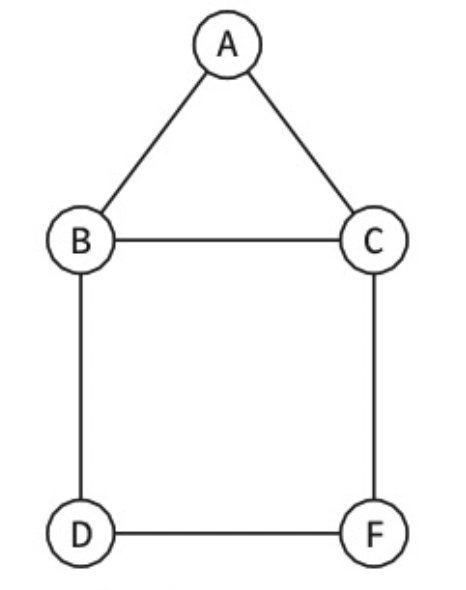
\includegraphics[keepaspectratio, width=0.22 \paperwidth]{GrundlagenInfo/DataScience/02_Graphen/Figures/4-graph.png}
        \end{figure}
        \begin{itemize}
            \item $V=\lrc{A,B,C,D,F}$
            \item $E=\lrc{\lrc{A,B},\lrc{A,C},\lrc{B,C},\lrc{B,D},\lrc{C,F},\lrc{D,F}}$
        \end{itemize}
    \end{itemize}

\end{frame}

\begin{frame}{\emoji{person-walking} Wege und Spaziergänge}
    \begin{itemize}
        \item Ein \tib{Weg} oder ein \tib{Spaziergang} in einem Graphen $G=(V,E)$ besteht aus einer Folge benachbarter Knoten, die miteinander verbunden werden
        \begin{itemize}
            \item Z.B. im Graph unten: $A,B,C,F,D$
            \item Wir sagen dem ersten und letzten Knoten in diesem Weg ($A$ und $D$) \tib{Endknoten}
            \begin{figure}
                \centering
                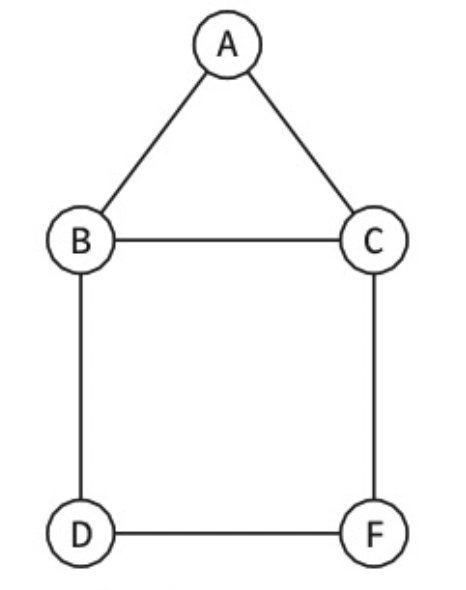
\includegraphics[keepaspectratio, width=0.2 \paperwidth]{GrundlagenInfo/DataScience/02_Graphen/Figures/4-graph.png}
            \end{figure}
        \end{itemize}
        \only<2->{
        \item Wir nennen einen Weg \tib{Kreis}, wenn die Endknoten gleich sind
        \begin{itemize}
            \item Z.B. $A,C,F,D,B,A$
            \item Ein Kreis ist \tib{einfach}, wenn ausser dem Endknoten kein anderer Knoten zweimal vorkommt
        \end{itemize}
        }
    \end{itemize}
\end{frame}

\begin{frame}{Spezielle Wege \emoji{motorway}}
\begin{itemize}
    \item Ein \tib{Euler'scher Weg} ist ein Weg, der alle Kanten eines Graphen genau einmal durchläuft. Graphen, die einen solchen Weg besitzen, nennen wir \tib{Euler'sche Graphen}
    % TODO Bild zu Königsberger Brückenproblem hinzufügen
    \item Ein \tib{Hamilton'scher Weg} ist ein einfacher Weg zwischen zwei Knoten eines Graphen, bei dem alle Knoten des Graphen enthalten sind.
 \end{itemize}
 \begin{figure}
     \centering
 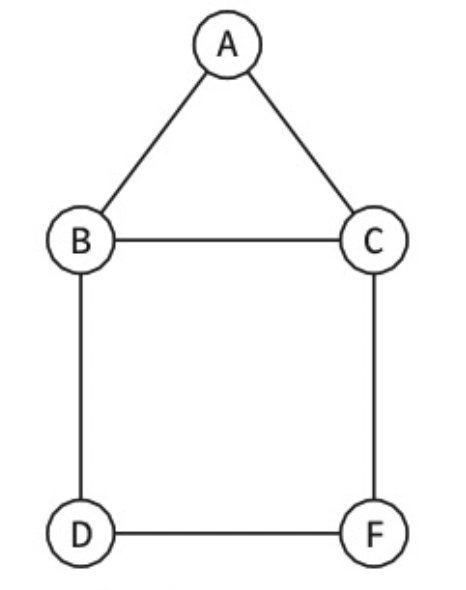
\includegraphics[keepaspectratio, width=0.18 \paperwidth]{GrundlagenInfo/DataScience/02_Graphen/Figures/4-graph.png}
 \end{figure}
 $\rightarrow$ Suchen Sie Euler'sche Wege/Kreise und Hamilton'sche Wege/Kreise in diesem Graph
    
\end{frame}

\begin{frame}{Zusammenhängende Graphen}
    \begin{itemize}[<+->]
        \item Ein Graph ist \tib{zusammenhängend}, wenn es zwischen jedem paar von Knoten mindestens einen Weg gibt.
        \item Wenn zwei Knoten A und B miteinander Verbunden sind $\lr{\exists\lrc{A, B}}$, dann heissen sie \tib{Nachbarn}    
        \item Der \textbf{Grad eines Knotens} $x \in V$, bezeichnet als $\deg(x)$, ist die Anzahl der mit x verbundenen Kanten
        \item Der \textbf{Grad eines Graphen} $G$, bezeichnet als $\deg(G)$, ist das Maximum der Grade aller Knoten im Graphen
    \end{itemize}
    \begin{figure}
        \centering
        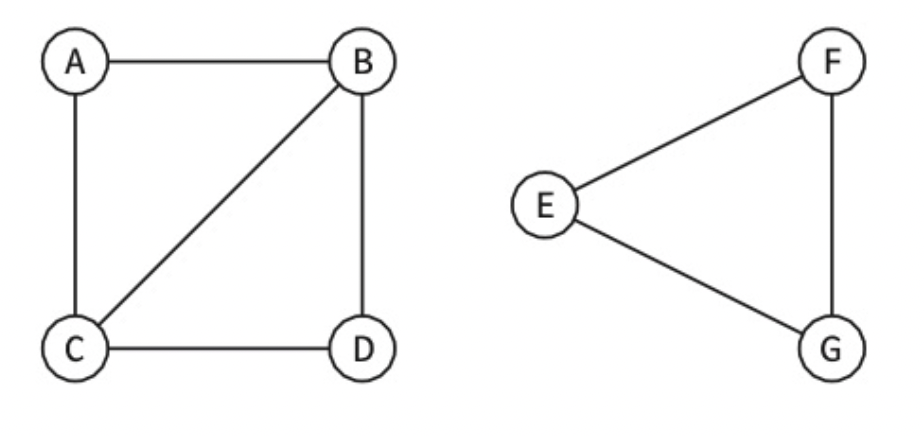
\includegraphics[keepaspectratio, width=0.35 \paperwidth]{GrundlagenInfo/DataScience/02_Graphen/Figures/4-graph-zusammenhaengend.png}
    \end{figure}
\end{frame}

\begin{frame}{Färbung von Graphen}
    \begin{itemize}[<+->]
        \item Die \tib{Färbung eines Graphen} erfolgt so, dass benachbarte Knoten immer unterschiedliche Farben haben. Ein Graph $G$ mit $k$ Farben heisst demnach \tib{k-färbbar}.
        \begin{figure}
            \centering
            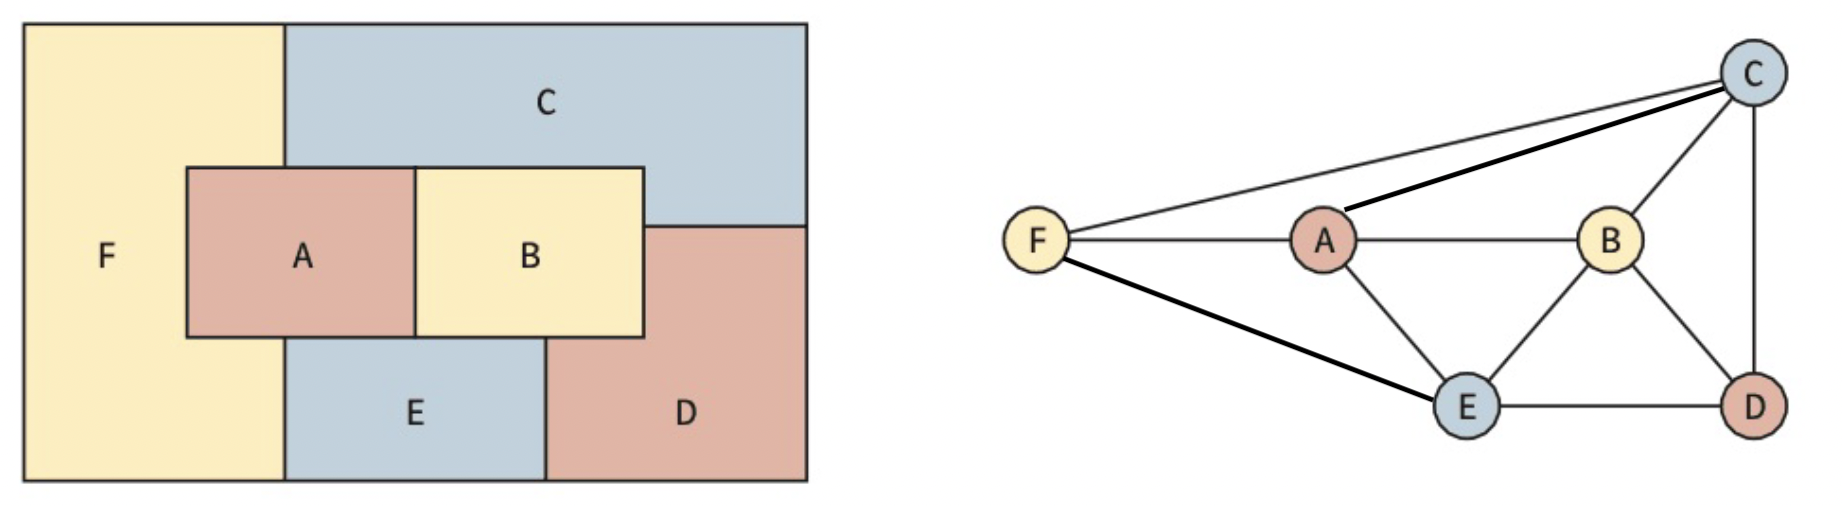
\includegraphics[keepaspectratio, width=0.6 \paperwidth]{GrundlagenInfo/DataScience/02_Graphen/Figures/4-graph-farbe.png}
        \end{figure}
        \item Ein \tib{vollständiger Graph} ist ein Graph von $n$ Knoten, in dem jeder Knoten mit jedem anderen Knoten verbunden ist 
        $$\forall x\in V:\quad \deg(x)=n-1$$
        \begin{figure}
            \centering
            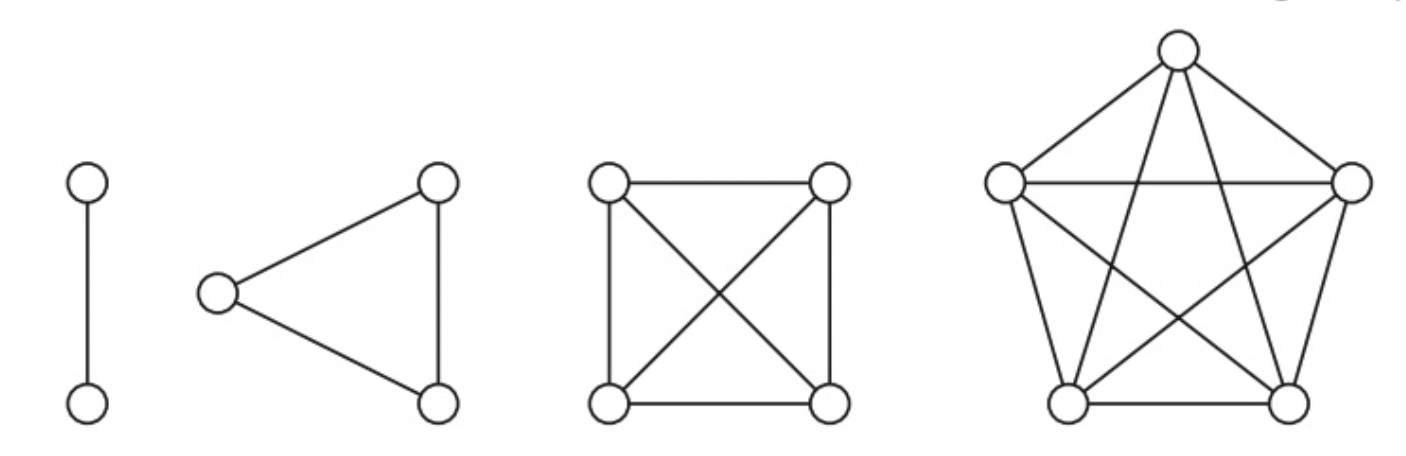
\includegraphics[keepaspectratio, width=0.45 \paperwidth]{GrundlagenInfo/DataScience/02_Graphen/Figures/4-graph-vollstaendig.png}
        \end{figure}
    \end{itemize}
\end{frame}

\begin{frame}{Planare Darstellung von Graphen}
    \begin{itemize}[<+->]
        \item Ein Graph ist \tib{planar} dargestellt, wenn keine Knoten sich überkreuzen.
        \begin{figure}
            \centering
            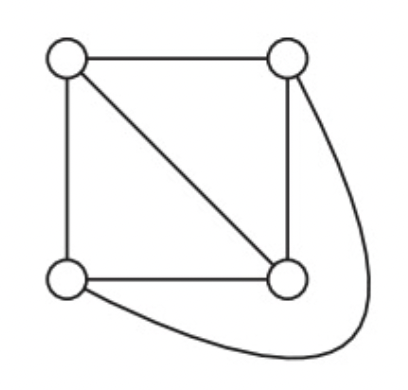
\includegraphics[keepaspectratio, width=0.2 \paperwidth]{GrundlagenInfo/DataScience/02_Graphen/Figures/4-graph-planar.png}
        \end{figure}
    \end{itemize}
\end{frame}

\begin{frame}[fragile]{Aufgaben}
\begin{enumerate}
    \item Aufgabe 1.38
    \item Aufgabe 1.39 a, c und d (Aufgabe b ignorieren, Fehler im Buch)
    \item Lesen Sie Beispiel 1.6 (Korrektur: beim Graph unten rechts sollten Kanten \textbf{F und E} sowie \textbf{A und C} miteinander verbunden sein)
    \item Aufgabe 1.42
    \item Aufgabe 1.44
    \item Aufgabe 1.45
    \item Aufgabe 1.48
    \item \textit{Challenge}: Aufgabe, 1.40, 1.47 und 1.49
\end{enumerate}
\vfill
\begin{center}
    Viel Erfolg!\\
    \emoji{deciduous-tree}\emoji{person-walking}\emoji{deciduous-tree}
\end{center}
\end{frame}